%---------------
%╔═╗╔═╗╔╦╗╦ ╦╔═╗
%╚═╗║╣  ║ ║ ║╠═╝
%╚═╝╚═╝ ╩ ╚═╝╩  
%---------------
\documentclass[12pt,oneside,a4paper]{report}

% DOCUMENT SETUP
\usepackage[left=3cm, 
			right=2.5cm, 
			top=2.5cm, 
			bottom=2.5cm, 
			includehead, 
			includefoot]{geometry}

% line spacing
\usepackage{setspace}
\setstretch{1,25} % 15/12 --> 1.25

%de­fines Adobe Times Ro­man as de­fault text font
\usepackage{mathptmx}
\usepackage{times} % needed for acronym package

%PDF linking package
\usepackage[hidelinks]{hyperref}

% Language Setup
\usepackage[ngerman]{babel}
% language specific bibliography style
\usepackage[numbers]{natbib}
\usepackage[fixlanguage]{babelbib}
\selectbiblanguage{german}
% bliographystyle setup
% default style names: apalike alphadin ieeetr IEEEtranSN apalike2 alphadin 
% babel specific: babplain, babplai3, babalpha, babunsrt, bababbrv, bababbr3 unsrt 
\bibliographystyle{unsrturl}

% encoding setup
% T1 font encoding for languages that use a latin alphabet
\usepackage[T1]{fontenc} 

% enhanced input encoding handling - utf8 for äÄüÜöÖß...
\usepackage[utf8]{inputenc}
%\usepackage{ucs}%utf8x suppart

% after babel - set chapter string
\AtBeginDocument{\renewcommand{\chaptername}{}}

% enumeration
\usepackage{enumitem}
% tabular extension tabularx
\usepackage{tabularx}

% math packages
\usepackage{amsmath}
\usepackage{nicefrac}
\usepackage{amsthm}
\usepackage{amsbsy}
\usepackage{amssymb}
\usepackage{amsfonts}
\usepackage{MnSymbol}

% patches for latex
\usepackage{fixltx2e}

%special characters
\usepackage{amssymb}
\usepackage{upgreek,textgreek}

% acronym package
\usepackage[printonlyused, footnote]{acronym}

% breakable text in \seqsplit{}
\usepackage{seqsplit}

% \textmu
\usepackage{textcomp}

% package provides a way to compile sections of a document using the same preamble as the main document
\usepackage{subfiles}

% driver-independent color extension - used by listings,tabularx
\usepackage[usenames,dvipsnames,table,xcdraw]{xcolor}

% -- SYNTAX HIGHLIGHTING --
\usepackage{listings}
%% bash command line Syntax Highlighting
\lstdefinestyle{BASH_CMD}{ 
  columns=fullflexible,            % copy pasteable listings
  language=bash,
  basicstyle=\small\sffamily,
  basicstyle   = \small \ttfamily,
  keywordstyle = [1]\small \ttfamily,
  keywordstyle = [2]\small \ttfamily,
  commentstyle = \small \ttfamily,
  numbers=none,
  captionpos=b, 
  breaklines=true,
  numberstyle=\tiny,
  numbersep=3pt,
  frame=tlrb,
  columns=fullflexible,
  backgroundcolor=\color{white!20},
  linewidth=\linewidth,
  literate=                        % replace in code
     {Ö}{{\"O}}1
     {Ä}{{\"A}}1
     {Ü}{{\"U}}1
     {ß}{{\ss}}2
     {ü}{{\"u}}1
     {ä}{{\"a}}1
     {ö}{{\"o}}1
}
 % adds style BASH_CMD
%% Matlab Syntax Highlighting
\colorlet{keyword}{blue!100!black!80}
\colorlet{STD}{Lavender}
\colorlet{comment}{green!90!black!90}
\definecolor{mygreen}{rgb}{0,0.6,0}
\definecolor{mygray}{rgb}{0.5,0.5,0.5}
\definecolor{mymauve}{rgb}{0.58,0,0.82}


\lstdefinestyle{BASH_SCRIPT}{ 
  language     = bash,
  basicstyle   = \footnotesize \ttfamily,
  keywordstyle = [1]\color{keyword}\bfseries,
  keywordstyle = [2]\color{STD}\bfseries,
  commentstyle = \color{mygreen}\itshape,
  backgroundcolor=\color{white},   % choose the background color; you must add \usepackage{color} 
  columns=fullflexible,            % copy pasteable listings
                                   % or \usepackage{xcolor}
  basicstyle=\footnotesize,        % the size of the fonts that are used for the code
  breakatwhitespace=false,         % sets if automatic breaks should only happen at whitespace
  breaklines=true,                 % sets automatic line breaking
  captionpos=b,                    % sets the caption-position to bottom
  extendedchars=true,              % lets you use non-ASCII characters; for 8-bits encodings only,
                                   % does not work with UTF-8
  frame=single,                    % adds a frame around the code
  keepspaces=true,                 % keeps spaces in text, useful for keeping indentation of code
                                   % (possibly needs columns=flexible)
  numbers=left,                    % where to put the line-numbers; possible values are 
                                   % (none, left, right)
  numbersep=5pt,                   % how far the line-numbers are from the code
  numberstyle=\tiny\color{mygray}, % the style that is used for the line-numbers
  rulecolor=\color{black},         % if not set, the frame-color may be changed on line-breaks
                                   % within not-black text (e.g. comments (green here))
  showspaces=false,                % show spaces everywhere adding particular underscores; it
  	                               % overrides 'showstringspaces'
  showstringspaces=false,          % underline spaces within strings only
  showtabs=false,                  % show tabs within strings adding particular underscores
  stepnumber=1,                    % the step between two line-numbers. If it's 1, each line 
                                   % will be numbered
  stringstyle=\color{mymauve},     % string literal style
  tabsize=2,                       % sets default tabsize to 2 spaces
  title=\lstname,                  % set title name
  literate=                        % replace in code
     {Ö}{{\"O}}1
     {Ä}{{\"A}}1
     {Ü}{{\"U}}1
     {ß}{{\ss}}2
     {ü}{{\"u}}1
     {ä}{{\"a}}1
     {ö}{{\"o}}1
} % adds style BASH_SCRIPT
% Matlab Syntax Highlighting
\colorlet{keyword}{blue!100!black!80}
\colorlet{STD}{red}
\colorlet{comment}{green!90!black!90}
\definecolor{mygreen}{rgb}{0,0.6,0}
\definecolor{mygray}{rgb}{0.5,0.5,0.5}
\definecolor{mymauve}{rgb}{0.58,0,0.82}


\lstdefinestyle{LATEX}{ 
  language     = [LaTeX]{TeX},
  basicstyle   = \footnotesize \ttfamily,
  keywordstyle = [1]\color{keyword}\bfseries,
  keywordstyle = [2]\color{comment}\bfseries,
  commentstyle = \color{mygray}\itshape,
  %backgroundcolor=\color{white},   % choose the background color; you must add \usepackage{color} 
                                   % or \usepackage{xcolor}
  basicstyle=\footnotesize,        		   % the size of the fonts that are used for the code
  breakatwhitespace=false,         % sets if automatic breaks should only happen at whitespace
  columns=fullflexible,            % copy pasteable listings
  breaklines=true,                 % sets automatic line breaking
  captionpos=c,                    % sets the caption-position to bottom
  extendedchars=true,              % lets you use non-ASCII characters; for 8-bits encodings only,
                                   % does not work with UTF-8
  frame=single,                    % adds a frame around the code
  keepspaces=true,                 % keeps spaces in text, useful for keeping indentation of code
                                   % (possibly needs columns=flexible)
  numbers=left,                    % where to put the line-numbers; possible values are 
                                   % (none, left, right)
  numbersep=4pt,                   % how far the line-numbers are from the code
  numberstyle=\tiny\color{mygray}, % the style that is used for the line-numbers
  rulecolor=\color{black},         % if not set, the frame-color may be changed on line-breaks
                                   % within not-black text (e.g. comments (green here))
  showspaces=false,                % show spaces everywhere adding particular underscores; it
  	                               % overrides 'showstringspaces'
  showstringspaces=false,          % underline spaces within strings only
  showtabs=false,                  % show tabs within strings adding particular underscores
  stepnumber=1,                    % the step between two line-numbers. If it's 1, each line 
                                   % will be numbered
  stringstyle=\color{mymauve},     % string literal style
  tabsize=2,                       % sets default tabsize to 2 spaces
  title=\lstname,                  % set title name
  literate=                        % replace in code
     {Ö}{{\"O}}1
     {Ä}{{\"A}}1
     {Ü}{{\"U}}1
     {ß}{{\ss}}2
     {ü}{{\"u}}1
     {ä}{{\"a}}1
     {ö}{{\"o}}1
} % adds style LATEX
%% Matlab Syntax Highlighting
\colorlet{keyword}{blue!100!black!80}
\colorlet{STD}{Lavender}
\colorlet{comment}{green!90!black!90}
\definecolor{mygreen}{rgb}{0,0.6,0}
\definecolor{mygray}{rgb}{0.5,0.5,0.5}
\definecolor{mymauve}{rgb}{0.58,0,0.82}


\lstdefinestyle{MATLAB}{ 
  language     = Matlab,
  basicstyle   = \footnotesize \ttfamily,
  keywordstyle = [1]\color{keyword}\bfseries,
  keywordstyle = [2]\color{STD}\bfseries,
  commentstyle = \color{mygreen}\itshape,
  backgroundcolor=\color{white},   % choose the background color; you must add \usepackage{color} 
                                   % or \usepackage{xcolor}
  basicstyle=\footnotesize,        % the size of the fonts that are used for the code
  breakatwhitespace=false,         % sets if automatic breaks should only happen at whitespace
  columns=fullflexible,            % copy pasteable listings
  breaklines=false,                % sets automatic line breaking
  captionpos=c,                    % sets the caption-position to bottom
  extendedchars=true,              % lets you use non-ASCII characters; for 8-bits encodings only,
                                   % does not work with UTF-8
  frame=single,                    % adds a frame around the code
  keepspaces=true,                 % keeps spaces in text, useful for keeping indentation of code
                                   % (possibly needs columns=flexible)
  numbers=left,                    % where to put the line-numbers; possible values are 
                                   % (none, left, right)
  numbersep=5pt,                   % how far the line-numbers are from the code
  numberstyle=\tiny\color{mygray}, % the style that is used for the line-numbers
  rulecolor=\color{black},         % if not set, the frame-color may be changed on line-breaks
                                   % within not-black text (e.g. comments (green here))
  showspaces=false,                % show spaces everywhere adding particular underscores; it
  	                               % overrides 'showstringspaces'
  showstringspaces=false,          % underline spaces within strings only
  showtabs=false,                  % show tabs within strings adding particular underscores
  stepnumber=1,                    % the step between two line-numbers. If it's 1, each line 
                                   % will be numbered
  stringstyle=\color{mymauve},     % string literal style
  tabsize=2,                       % sets default tabsize to 2 spaces
  title=\lstname,                  % set title name
  literate=                        % replace in code
     {Ö}{{\"O}}1
     {Ä}{{\"A}}1
     {Ü}{{\"U}}1
     {ß}{{\ss}}2
     {ü}{{\"u}}1
     {ä}{{\"a}}1
     {ö}{{\"o}}1
} % adds style MATLAB
% Matlab Syntax Highlighting
\colorlet{keyword}{blue!100!black!80}
\colorlet{STD}{Lavender}
\colorlet{comment}{green!90!black!90}
\definecolor{mygreen}{rgb}{0,0.6,0}
\definecolor{mygray}{rgb}{0.5,0.5,0.5}
\definecolor{mymauve}{rgb}{0.58,0,0.82}


\lstdefinestyle{PYTHON}{ 
  language     = Python,
  basicstyle   = \footnotesize \ttfamily,
  keywordstyle = [1]\color{keyword}\bfseries,
  keywordstyle = [2]\color{STD}\bfseries,
  commentstyle = \color{mygreen}\itshape,
  backgroundcolor=\color{white},   % choose the background color; you must add \usepackage{color} 
                                   % or \usepackage{xcolor}
  basicstyle=\footnotesize,        % the size of the fonts that are used for the code
  columns=fullflexible,            % copy pasteable listings
  breakatwhitespace=false,         % sets if automatic breaks should only happen at whitespace
  breaklines=false,                % sets automatic line breaking
  captionpos=c,                    % sets the caption-position to bottom
  extendedchars=true,              % lets you use non-ASCII characters; for 8-bits encodings only,
                                   % does not work with UTF-8
  frame=single,                    % adds a frame around the code
  keepspaces=true,                 % keeps spaces in text, useful for keeping indentation of code
                                   % (possibly needs columns=flexible)
  numbers=left,                    % where to put the line-numbers; possible values are 
                                   % (none, left, right)
  numbersep=5pt,                   % how far the line-numbers are from the code
  numberstyle=\tiny\color{mygray}, % the style that is used for the line-numbers
  rulecolor=\color{black},         % if not set, the frame-color may be changed on line-breaks
                                   % within not-black text (e.g. comments (green here))
  showspaces=false,                % show spaces everywhere adding particular underscores; it
  	                               % overrides 'showstringspaces'
  showstringspaces=false,          % underline spaces within strings only
  showtabs=false,                  % show tabs within strings adding particular underscores
  stepnumber=1,                    % the step between two line-numbers. If it's 1, each line 
                                   % will be numbered
  stringstyle=\color{mymauve},     % string literal style
  tabsize=2,                       % sets default tabsize to 2 spaces
  title=\lstname,                  % set title name
  literate=                        % replace in code
     {Ö}{{\"O}}1
     {Ä}{{\"A}}1
     {Ü}{{\"U}}1
     {ß}{{\ss}}2
     {ü}{{\"u}}1
     {ä}{{\"a}}1
     {ö}{{\"o}}1
} % adds style PYTHON
%% Matlab Syntax Highlighting
\colorlet{keyword}{blue!100!black!80}
\colorlet{STD}{Lavender}
\colorlet{comment}{green!90!black!90}
\definecolor{mygreen}{rgb}{0,0.6,0}
\definecolor{mygray}{rgb}{0.5,0.5,0.5}
\definecolor{mymauve}{rgb}{0.58,0,0.82}


\lstdefinestyle{CPP}{ 
  language     = C++,
  basicstyle   = \footnotesize \ttfamily,
  keywordstyle = [1]\color{keyword}\bfseries,
  keywordstyle = [2]\color{STD}\bfseries,
  commentstyle = \color{mygreen}\itshape,
  backgroundcolor=\color{white},   % choose the background color; you must add \usepackage{color} 
                                   % or \usepackage{xcolor}
  columns=fullflexible,            % copy pasteable listings
  basicstyle=\footnotesize,        % the size of the fonts that are used for the code
  breakatwhitespace=false,         % sets if automatic breaks should only happen at whitespace
  breaklines=false,                % sets automatic line breaking
  captionpos=c,                    % sets the caption-position to bottom
  extendedchars=true,              % lets you use non-ASCII characters; for 8-bits encodings only,
                                   % does not work with UTF-8
  frame=single,                    % adds a frame around the code
  keepspaces=true,                 % keeps spaces in text, useful for keeping indentation of code
                                   % (possibly needs columns=flexible)
  numbers=left,                    % where to put the line-numbers; possible values are 
                                   % (none, left, right)
  numbersep=5pt,                   % how far the line-numbers are from the code
  numberstyle=\tiny\color{mygray}, % the style that is used for the line-numbers
  rulecolor=\color{black},         % if not set, the frame-color may be changed on line-breaks
                                   % within not-black text (e.g. comments (green here))
  showspaces=false,                % show spaces everywhere adding particular underscores; it
  	                               % overrides 'showstringspaces'
  showstringspaces=false,          % underline spaces within strings only
  showtabs=false,                  % show tabs within strings adding particular underscores
  stepnumber=1,                    % the step between two line-numbers. If it's 1, each line 
                                   % will be numbered
  stringstyle=\color{mymauve},     % string literal style
  tabsize=2,                       % sets default tabsize to 2 spaces
  title=\lstname,                  % set title name
  literate=                        % replace in code
     {Ö}{{\"O}}1
     {Ä}{{\"A}}1
     {Ü}{{\"U}}1
     {ß}{{\ss}}2
     {ü}{{\"u}}1
     {ä}{{\"a}}1
     {ö}{{\"o}}1
} % adds style CPP
%% Matlab Syntax Highlighting
\colorlet{keyword}{blue!100!black!80}
\colorlet{STD}{Lavender}
\colorlet{comment}{green!90!black!90}
\definecolor{mygreen}{rgb}{0,0.6,0}
\definecolor{mygray}{rgb}{0.5,0.5,0.5}
\definecolor{mymauve}{rgb}{0.58,0,0.82}


\lstdefinestyle{C}{ 
  language     = C,
  basicstyle   = \footnotesize \ttfamily,
  keywordstyle = [1]\color{keyword}\bfseries,
  keywordstyle = [2]\color{STD}\bfseries,
  commentstyle = \color{mygreen}\itshape,
  backgroundcolor=\color{white},   % choose the background color; you must add \usepackage{color} 
  columns=fullflexible,            % copy pasteable listings
                                   % or \usepackage{xcolor}
  basicstyle=\footnotesize,        % the size of the fonts that are used for the code
  breakatwhitespace=false,         % sets if automatic breaks should only happen at whitespace
  breaklines=false,                % sets automatic line breaking
  captionpos=c,                    % sets the caption-position to bottom
  extendedchars=true,              % lets you use non-ASCII characters; for 8-bits encodings only,
                                   % does not work with UTF-8
  frame=single,                    % adds a frame around the code
  keepspaces=true,                 % keeps spaces in text, useful for keeping indentation of code
                                   % (possibly needs columns=flexible)
  numbers=left,                    % where to put the line-numbers; possible values are 
                                   % (none, left, right)
  numbersep=5pt,                   % how far the line-numbers are from the code
  numberstyle=\tiny\color{mygray}, % the style that is used for the line-numbers
  rulecolor=\color{black},         % if not set, the frame-color may be changed on line-breaks
                                   % within not-black text (e.g. comments (green here))
  showspaces=false,                % show spaces everywhere adding particular underscores; it
  	                               % overrides 'showstringspaces'
  showstringspaces=false,          % underline spaces within strings only
  showtabs=false,                  % show tabs within strings adding particular underscores
  stepnumber=1,                    % the step between two line-numbers. If it's 1, each line 
                                   % will be numbered
  stringstyle=\color{mymauve},     % string literal style
  tabsize=2,                       % sets default tabsize to 2 spaces
  title=\lstname,                  % set title name
  literate=                        % replace in code
     {Ö}{{\"O}}1
     {Ä}{{\"A}}1
     {Ü}{{\"U}}1
     {ß}{{\ss}}2
     {ü}{{\"u}}1
     {ä}{{\"a}}1
     {ö}{{\"o}}1
} % adds style C
%% JSON Syntax Highlighting
\colorlet{keyword}{blue!100!black!80}
\colorlet{STD}{Lavender}
\colorlet{comment}{green!90!black!90}
\definecolor{mygreen}{rgb}{0,0.6,0}
\definecolor{mygray}{rgb}{0.5,0.5,0.5}
\definecolor{mymauve}{rgb}{0.58,0,0.82}

\newcommand\JSONnumbervaluestyle{\color{blue}}
\newcommand\JSONstringvaluestyle{\color{red}}

\newif\ifcolonfoundonthisline

\makeatletter

\lstdefinelanguage{json}
{
  showstringspaces    = false,
  keywords            = {false,true},
  alsoletter          = 0123456789.,
  morestring          = [s]{"}{"},
  morestring          = [s]{'}{'},
  stringstyle         = \ifcolonfoundonthisline\JSONstringvaluestyle\fi,
  MoreSelectCharTable =%
    \lst@DefSaveDef{`:}\colon@json{\processColon@json},
  basicstyle          = \ttfamily,
  keywordstyle        = \ttfamily\bfseries,
}

% flip the switch if a colon is found in Pmode
\newcommand\processColon@json{
  \colon@json%
  \ifnum\lst@mode=\lst@Pmode%
    \global\colonfoundonthislinetrue%
  \fi
}

\lst@AddToHook{Output}{%
  \ifcolonfoundonthisline%
    \ifnum\lst@mode=\lst@Pmode%
      \def\lst@thestyle{\JSONnumbervaluestyle}%
    \fi
  \fi
  %override by keyword style if a keyword is detected!
  \lsthk@DetectKeywords% 
}

% reset the switch at the end of line
\lst@AddToHook{EOL}%
  {\global\colonfoundonthislinefalse}

\makeatother



\lstdefinestyle{JSON}{ 
  language     = json,
  basicstyle   = \footnotesize \ttfamily,
  keywordstyle = [1]\color{keyword}\bfseries,
  keywordstyle = [2]\color{STD}\bfseries,
  commentstyle = \color{mygreen}\itshape,
  backgroundcolor=\color{white},   % choose the background color; you must add \usepackage{color} 
                                   % or \usepackage{xcolor}
  basicstyle=\footnotesize,        % the size of the fonts that are used for the code
  columns=fullflexible,            % copy pasteable listings
  breakatwhitespace=false,         % sets if automatic breaks should only happen at whitespace
  breaklines=false,                % sets automatic line breaking
  captionpos=c,                    % sets the caption-position to bottom
  extendedchars=true,              % lets you use non-ASCII characters; for 8-bits encodings only,
                                   % does not work with UTF-8
  frame=single,                    % adds a frame around the code
  keepspaces=true,                 % keeps spaces in text, useful for keeping indentation of code
                                   % (possibly needs columns=flexible)
  numbers=left,                    % where to put the line-numbers; possible values are 
                                   % (none, left, right)
  numbersep=5pt,                   % how far the line-numbers are from the code
  numberstyle=\tiny\color{mygray}, % the style that is used for the line-numbers
  rulecolor=\color{black},         % if not set, the frame-color may be changed on line-breaks
                                   % within not-black text (e.g. comments (green here))
  showspaces=false,                % show spaces everywhere adding particular underscores; it
  	                               % overrides 'showstringspaces'
  showstringspaces=false,          % underline spaces within strings only
  showtabs=false,                  % show tabs within strings adding particular underscores
  stepnumber=1,                    % the step between two line-numbers. If it's 1, each line 
                                   % will be numbered
  stringstyle=\color{mymauve},     % string literal style
  tabsize=2,                       % sets default tabsize to 2 spaces
  title=\lstname,                  % set title name
  literate=                        % replace in code
     {Ö}{{\"O}}1
     {Ä}{{\"A}}1
     {Ü}{{\"U}}1
     {ß}{{\ss}}2
     {ü}{{\"u}}1
     {ä}{{\"a}}1
     {ö}{{\"o}}1
} % adds style JSON

% HEADLINE CFG
\usepackage{fancyhdr} % Headers and footers
\usepackage{lastpage}
\usepackage{nopageno}
\setlength{\headheight}{1.5cm}
\pagestyle{fancy} % All pages have headers and footers
\fancyhead{} % Blank out the default header
\fancyfoot{} % Blank out the default footer
\fancyhead[L]{}
\fancyhead[C]{}
\fancyhead[R]{}
\fancyfoot[L]{}
\fancyfoot[C]{\thepage}
\fancyfoot[R]{}
% override plain page style for \part, \chapter or 
% \maketitle, which implicit specifies plain page style
\fancypagestyle{plain} 
{
	\fancyhead[L]{}
	\fancyhead[C]{}
	\fancyhead[R]{}
	\fancyfoot[L]{}
	\fancyfoot[C]{\thepage}
	\fancyfoot[R]{}
}
% set list pagestyle
\fancypagestyle{lists} 
{
	\fancyhead[L]{}
	\fancyhead[C]{}
	\fancyhead[R]{}
	\fancyfoot[L]{}
	\fancyfoot[C]{\thepage}
	\fancyfoot[R]{}
}

\renewcommand{\chaptermark}[1]{\markright{#1}{}}
\renewcommand{\sectionmark}[1]{\markright{#1}{}}
\renewcommand{\headrulewidth}{0pt}
\renewcommand{\footrulewidth}{0pt}

	
\usepackage{verbatim}
\usepackage{graphicx}
\usepackage{epstopdf}

% floating prevention packages
\usepackage{float}    % used with [H] positioning parameter
\usepackage{placeins} % \FloatBarrier 

% tikz packages
\usepackage{tikz}
\usepackage{caption}
\usepackage[list=true,listformat=simple]{subcaption}
\usepackage{standalone}
\usepackage{pgfplots}


% include only specified tex files - uncommend unneeded
\includeonly{preface/cover,
             preface/abstract,
             preface/tableofcontents,
             preface/listoffigures,
             preface/listoftables,
             preface/lstlistoflistings,
             appendix/bibliography}

%-------------------
%╔═╗╔╦╗╦═╗╦╔╗╔╔═╗╔═╗
%╚═╗ ║ ╠╦╝║║║║║ ╦╚═╗
%╚═╝ ╩ ╩╚═╩╝╚╝╚═╝╚═╝
%-------------------
\newcommand{\strLecture}{Signale, Systeme und Sensoren}
\newcommand{\strDate}{\today}
\newcommand{\strAuthorA}{M. Kieser}
\newcommand{\strAuthorB}{J. Altmeyer}
\newcommand{\strAuthorAEmail}{makieser@htwg-konstanz.de}
\newcommand{\strAuthorBEmail}{jualtmey@htwg-konstanz.de}
% Versuchsbeschreibung 
\newcommand{\strTopic}{Fourieranalyse und Akustik}
\newcommand{\strAbstract}{In diesem Versuch wird die Tonhöhe eines akustischen Signals und der Frequenzgang von zwei Lautsprechern ermittelt. Um die Tonhöhe eines Signals zu bestimmen, wird u.a. die Fourieranalyse verwendet. In dem dadurch entstandenen Spektrum lässt sich die Tonhöhe bzw. die Frequenz einfach ablesen. Im Ergebnis konnte eine Tonhöhe von 1923 Hz festgestellt werden. In dem jeweiligen Frequenzgang der beiden Lautsprecher zeigt sich, dass die Lautsprecher das Eingangssignal nicht linear wiedergeben. 
}
% hyperref customization
\hypersetup{
	pdftitle    ={\strTopic}, % title
	pdfsubject	={\strLecture}, % subject of the document
	pdfauthor	={\strAuthorA, \strAuthorB}, % author
	pdfkeywords	={}, % list of keywords
	pdfcreator	={}, % creator of the document
	pdfproducer	={}, % producer of the document
	colorlinks=false, % false: boxed links; true: colored links
	linkcolor=red, % color of internal links (change box color with linkbordercolor)
    citecolor=green, % color of links to bibliography
    filecolor=magenta, % color of file links
    urlcolor=cyan, % color of external links
	%bookmarks=true, % show bookmarks bar?
	unicode=true, % non-Latin characters in Acrobat’s bookmarks
	pdftoolbar=true, % show Acrobat’s toolbar?
	pdfmenubar=true, % show Acrobat’s menu?
    pdffitwindow=false, % window fit to page when opened
	pdfnewwindow=true % links in new PDF window
}

%-----------------------------------------
% ╔╗ ╔═╗╔═╗╦╔╗╔  ╔╦╗╔═╗╔═╗╦ ╦╔╦╗╔═╗╔╗╔╔╦╗ 
% ╠╩╗║╣ ║ ╦║║║║   ║║║ ║║  ║ ║║║║║╣ ║║║ ║  
% ╚═╝╚═╝╚═╝╩╝╚╝  ═╩╝╚═╝╚═╝╚═╝╩ ╩╚═╝╝╚╝ ╩  
%-----------------------------------------

\begin{document}
\pagenumbering{Roman} 

%\setcounter{section}{0}

\begin{titlepage}

\vspace*{-3.5cm}

\begin{flushleft}
\hspace*{-1cm} 
\includegraphics[width=15.7cm]{preface/htwg-logo}
\end{flushleft}

\vspace{1cm}

\begin{center}
	\large{
		\textbf{\strLecture} \\[2cm]
	}
	\Huge{
		\textbf{\strTopic} \\[2cm]
	}
	\Large{
		\textbf{\strAuthorA, \strAuthorB}} \\[3cm]
	\large{
		\textbf{} \\[2.3cm]
	}
	
	\large{
		\textbf{Konstanz, \strDate}
	}
\end{center}

\end{titlepage}
\thispagestyle{empty}




\begin{center}
{\Large \textbf{Zusammenfassung (Abstract)}}
\end{center}

\bigskip

\begin{center}
	\begin{tabular}{p{2.8cm}p{5cm}p{5cm}}
		Thema: & \multicolumn{2}{p{10cm}}{\raggedright\strTopic} \\
		 & & \\
		Autoren: & \strAuthorA & \href{mailto:\strAuthorAEmail}{\strAuthorAEmail} \\
		 & \strAuthorB & \href{mailto:\strAuthorBEmail}{\strAuthorBEmail} \\
		 & & \\
		Betreuer: & Prof. Dr. Matthias O. Franz & \href{mailto:mfranz@htwg-konstanz.de}{mfranz@htwg-konstanz.de} \\
		 &  Jürgen Keppler & \href{mailto:juergen.keppler@htwg-konstanz.de}{juergen.keppler@htwg-konstanz.de} \\
		 &  Martin Miller & \href{mailto:martin.miller@htwg-konstanz.de}{martin.miller@htwg-konstanz.de} \\
	\end{tabular}
\end{center}

\bigskip

\noindent
\strAbstract

\thispagestyle{lists}



\clearpage

%
% TABLE OF CONTENTS
%
\thispagestyle{lists}
%
% TABLE OF CONTENTS
%
\tableofcontents
\thispagestyle{plain}
\newpage

%
% Abbildungsverzeichnis
%
%
% Abbildungsverzeichnis
%
\phantomsection
\addcontentsline{toc}{chapter}{Abbildungsverzeichnis}
\listoffigures
\thispagestyle{lists}
\newpage

%
% Tabellenverzeichnis
%
%%
% Tabellenverzeichnis
%
\phantomsection
\addcontentsline{toc}{chapter}{Tabellenverzeichnis}
\listoftables
\thispagestyle{lists}
\newpage

%
% Listingverzeichnis
%
%
% Listingverzeichnis
%
\phantomsection
\renewcommand\lstlistingname{Listing}
\renewcommand\lstlistlistingname{Listingverzeichnis}
\lstlistoflistings
\addcontentsline{toc}{chapter}{Listingverzeichnis}
\thispagestyle{lists}
\newpage


%--------------------------
% ╔═╗╦ ╦╔═╗╔═╗╔╦╗╔═╗╦═╗╔═╗ 
% ║  ╠═╣╠═╣╠═╝ ║ ║╣ ╠╦╝╚═╗ 
% ╚═╝╩ ╩╩ ╩╩   ╩ ╚═╝╩╚═╚═╝ 
%--------------------------

\pagenumbering{arabic} 
\setcounter{page}{1}
%
% CHAPTER Einleitung
%
\chapter{Einleitung}
\label{chap:EINL}

In den folgenden Versuchen soll u. a. gezeigt werden, wie die Tonhöhe eines akustischen Signals am Beispiel einer Mundharmonika bestimmt werden kann. Dazu wird zum einen das aufgenommene Signal analysiert und zum anderen eine Fourieranalyse angewandt, um aus dem erhaltenem Spektrum die Tonhöhe feststellen zu können. 
Des weiteren wird der Frequenzgang von zwei Lautsprechern ermittelt und untersucht. Wie gut sind die Lautsprecher? Welche Frequenzen werden verstärkt oder abgeschwächt?
\paragraph{}
Diese Versuche basieren auf dem dritten Aufgabenblatt \cite{Franz2015p} aus der Vorlesung Signale Systeme und Sensoren.
%
% CHAPTER Versuch 1
%
\chapter{Versuch 1 - Bestimmung der Tonhöhe eines akustischen Signals}
\label{chap:VERSUCH_1}
Im nachfolgenden Versuch soll die Tonhöhe eines Akkustischen Signals gemessen werden. Dabei werden zwei verschiedene Verfahren zur Ermittlung der Tonhöhe bzw. Grundfrequenz durchgeführt. Zum einen durch direktes auslesen der Daten und zum anderen durch das Amplitudenspektrum mithilfe der Fouriertransformation.

\section{Fragestellung, Messprinzip, Aufbau, Messmittel}
\label{chap:VERSUCH_1_FRAGESTELLUNG}
Was ist die Tonhöhe bzw. Grundfrequenz eines akustischen Signals verursacht durch eine Mundharmonika?
Messprinzip ist aufgebaut aus einem Audiosensor in Form eines Mikrophons [Messmittel], welches an ein Oszilloskop angeschlossen ist, dass die eingehenden Informationen als Spannungswerte pro Zeit darstellt.
Der Aufbau des Versuchs besteht aus einer Mundharmonika, die einen Ton in das Mikrophon abgibt und dieser vom Oszilloskop aufgezeichnet wird.

\section{Messwerte}
\label{chap:VERSUCH_1_MESSWERTE}

Das aperiodische Signal von einem Mundharmonika Ton, der 25 ms aufgezeichnet wurde ist in Abbildung \ref{fig:SignalKomplet} zu sehen.

\begin{figure}[H]
	\centering\small
	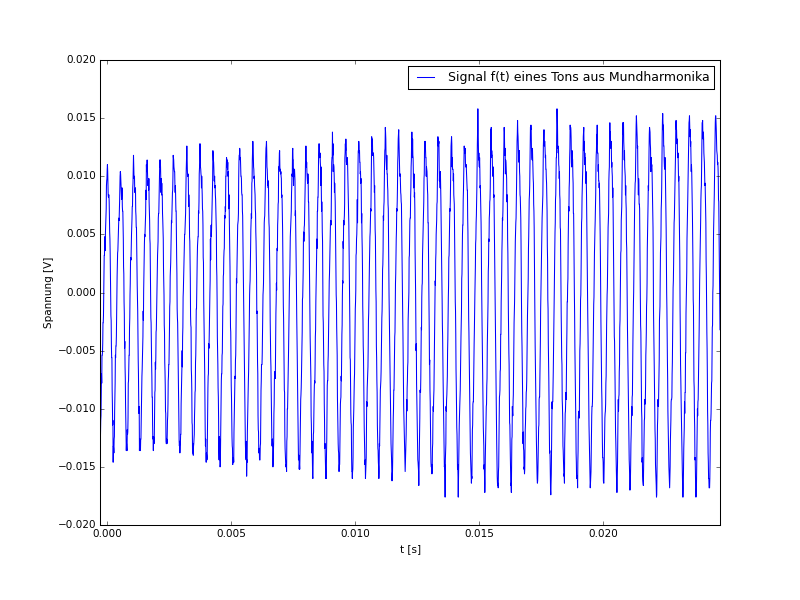
\includegraphics[width=\textwidth]{src/V1_Signal_komplet.png}
	\caption{Mundharmonika Signal von 25 ms Dauer}
	\label{fig:SignalKomplet}
\end{figure}

Zur Verdeutlichung des Signals ein vergrößerter Ausschnitt des Anfangs in Abbildung \ref{fig:SignalAusschnitt} .

\begin{figure}[H]
	\centering\small
	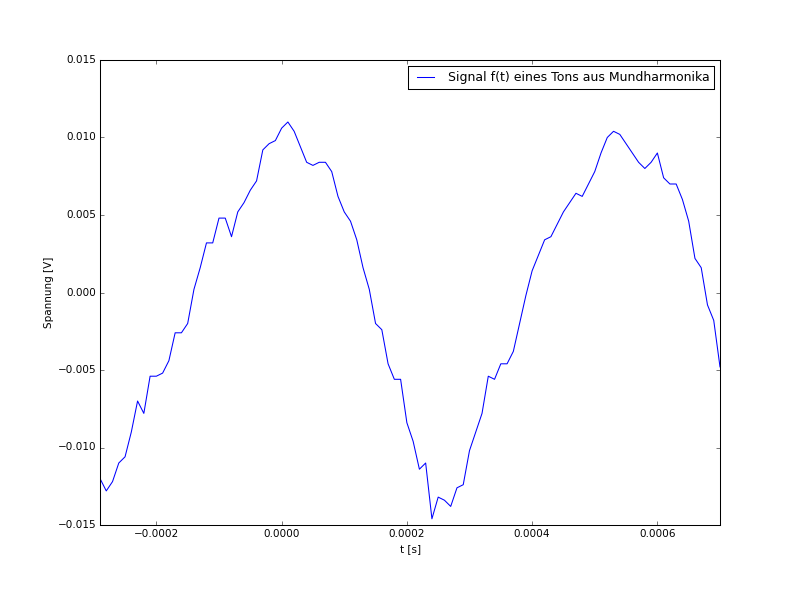
\includegraphics[width=\textwidth]{src/V1_Signal_grundfrequenz.png}
	\caption{Mundharmonika Signal Ausschnitt}
	\label{fig:SignalAusschnitt}
\end{figure}

\section{Auswertung}
\label{chap:VERSUCH_1_AUSWERTUNG}
Nachfolgend wird die Auswertung in zwei mögliche Ermittlungsverfahren unterteilt. \\

\textbf{1. ermitteln der Grundfrequenz und anderer Eckdaten durch direktes ablesen aus den Daten}\\
Die nachfolgenden Werte ergeben sich durch auslesen der Daten, die in Abbildung \ref{fig:SignalKomplet} dargestellt sind.  Die Grundperiode ermittelt sich aus auslesen der Zeit einer Periode aus den Daten. Hierfür wurde die Zeitdifferenz zwischen zwei maximal Ausschlägen gemessen. 
Die Grundfrequenz berechnet sich dann aus dem Kehrwert der Grundperiode. \\
\\
Grundperiode: 0.52 ms \\
Grundfrequenz: 1923 Hz \\
Signaldauer: 0.025 s \\
Abtastfrequenz: 100 kHz \\
Signallänge M: 2500 \\
Abtastintervall $\Delta t$: 0.00001 s \\

\textbf{2. ermitteln der Grundfrequenz mit Hilfe der Fouriertransformierten des Signals} \\
In Abbildung \ref{fig:Spektrum} ist das Amplitudenspektrum in Hertz abgebildet. Dies wurde aus dem Mundharmonika Signal mithilfe der Fouriertransformation erstellt. Die Berechnung der Ergebnisse ist dem Pythoncode in Listing \ref{lst:Code} Methode versuch1\_2 zu entnehmen.

\begin{figure}[H]
	\centering\small
	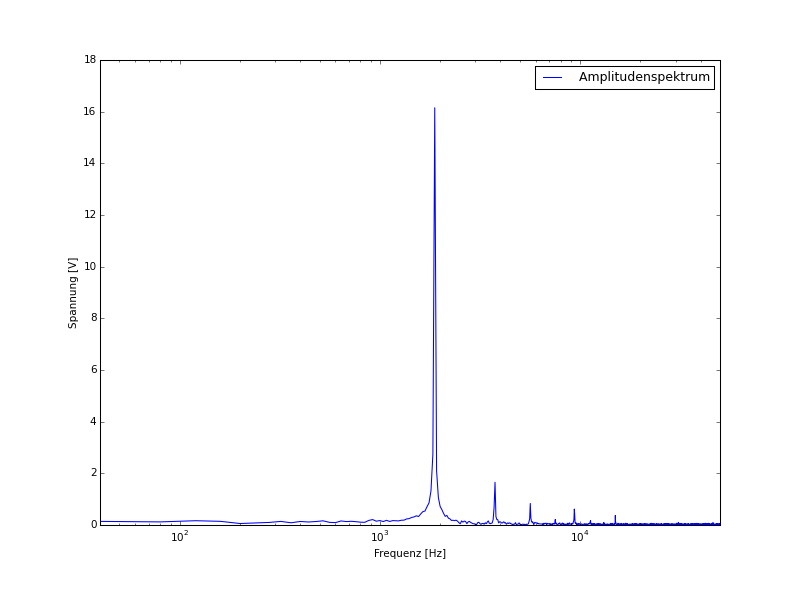
\includegraphics[width=\textwidth]{src/V1_2_Amplitudenspektrum.png}
	\caption{Amplitudenspektrum in Hertz (halblogarithmische Darstellung der Frequenz)}
	\label{fig:Spektrum}
\end{figure}

\section{Interpretation}
\label{chap:VERSUCH_1_INTERPRETATION}
Wie aus der Abbildung \ref{fig:Spektrum} zu erkennen ist, ist der Amplitudenausschlag bei ca. 2000 Hz besonders stark. Dies entspricht auch dem durch ablesen ermittelten Wert der Grundfrequenz von 1923 Hz. Somit weisen beide Ermittlungsverfahren das gleiche Ergebnis auf. Bei der Ermittlung über das Amplitudenspektrum kann man desweiteren aussagen über das ganze Spektrum machen. Hier zum Beispiel, dass noch ein Anteil von vielfachen der Grundfrequenz enthalten sind.

%
% CHAPTER Versuch 2
%
\chapter{Versuch 2 - Frequenzgang von Lautsprechern}
\label{chap:VERSUCH_2}

Dieser Versuch zeigt, wie der Frequenzgang eines Lautsprechers ermittelt werden kann.
Dazu werden zwei unterschiedlich große Lautsprecher verwendet.

\section{Fragestellung, Messprinzip, Aufbau, Messmittel}
\label{chap:VERSUCH_2_FRAGESTELLUNG}

Wie verändert ein Lautsprecher sein Eingangsignal? Welche Frequenzen werden verstärkt, abgeschwächt oder verzögert?
Um dies beantworten zu können, benötigt man den Frequenzgang des Lautsprechers.
\paragraph{}
Für diesen Versuch wurde ein Funktionsgenerator, ein Oszilloskop, zwei unterschiedlich große Lautsprecher und ein Mikrofon verwendet.
Der Funktionsgenerator ist mit dem Oszilloskop und einem Lautsprecher verbunden. Das Mikrofon ist jeweils zu diesem Lautsprecher hin ausgerichtet und auch mit dem Oszilloskop verbunden. Folgende Messungen wurden einmal für den großen und einmal für den kleinen Lautsprecher durchgeführt.
\paragraph{}
Mit dem Funktionsgenerator wird zunächst ein Sinussignal mit 100 Hz erzeugt.
Dieses Signal gibt der Lautsprecher wieder und das Mikrofon nimmt es auf.
Das original Signal des Funktionsgenerators und das Ausgangssignal des Lautsprechers werden nun auf dem Oszilloskop dargestellt.
Dadurch kann die Amplitude und die Phasenverschiebung des Ausgangssignals abgelesen werden.
Dies wird für die Frequenzen 200, 300, 400, 500, 700, 850 Hz, 1, 1.2, 1.5, 1.7, 2, 3, 4, 5, 6, 10 kHz wiederholt.


\section{Messwerte}
\label{chap:VERSUCH_2_MESSWERTE}

In Abbildung \ref{fig:LAUT_TIEF} und \ref{fig:LAUT_HOCH} sind die Ergebnisse der oben durchgeführten Messungen für die beiden Lautsprecher zu sehen. Es ist tabellarisch die Frequenz und die dazugehörige Amplitude und Phasenverschiebung eingetragen.

\section{Auswertung}
\label{chap:VERSUCH_2_AUSWERTUNG}

Die Messwerte wurden in Python übertragen und graphisch dargestellt (Listing \ref{lst:Code}). Abbildung \ref{fig:LAUT_TIEF_FREQUENZGANG} und \ref{fig:LAUT_HOCH_FREQUENZGANG} zeigen somit den Frequenzgang für den jeweiligen Lautsprecher. Die Spannung wurde in Dezibel und die Phase in Grad umgerechnet.


\begin{figure}
\centering\small
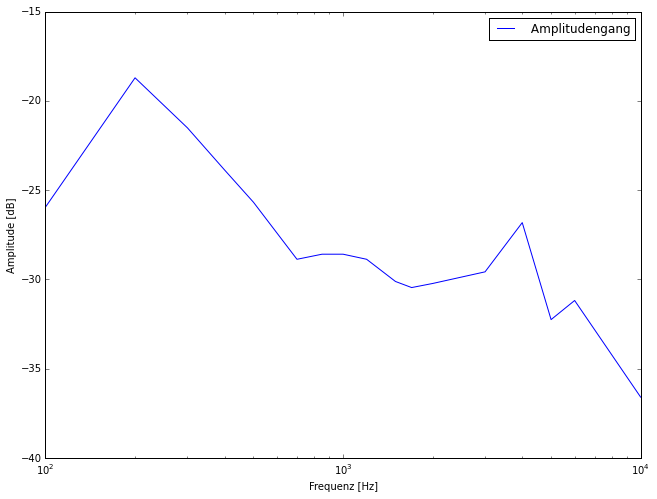
\includegraphics[scale=0.6]{src/AmplitudenspektrumLautsprecher1.png}
%\caption{Messwerte des kleinen Lautsprechers}
%\label{fig:LAUT_HOCH}
%\centering\small
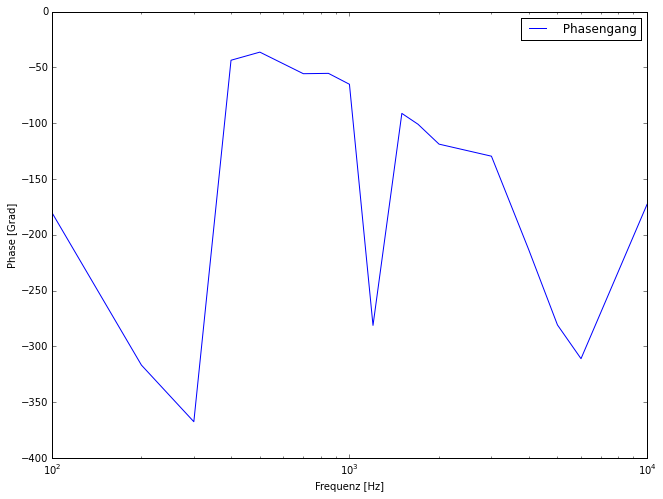
\includegraphics[scale=0.6]{src/PhasenverschiebungLautsprecher1.png}
\caption{Frequenzgang des großen Lautsprechers}
\label{fig:LAUT_TIEF_FREQUENZGANG}
\end{figure}

\begin{figure}
\centering\small
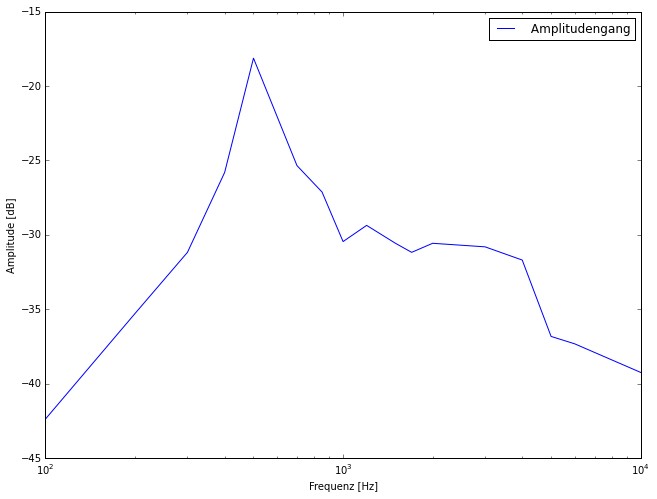
\includegraphics[scale=0.6]{src/AmplitudenspektrumLautsprecher2.png}
%\caption{Messwerte des kleinen Lautsprechers}
%\label{fig:LAUT_HOCH}
%\centering\small
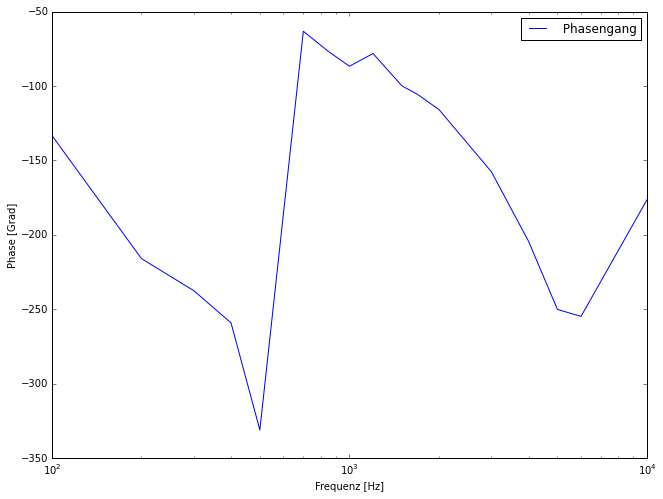
\includegraphics[scale=0.6]{src/PhasenverschiebungLautsprecher2.png}
\caption{Frequenzgang des kleinen Lautsprechers}
\label{fig:LAUT_HOCH_FREQUENZGANG}
\end{figure}

\section{Interpretation}
\label{chap:VERSUCH_2_INTERPRETATION}

Generell muss man sagen, dass nur der Frequenzbereich zwischen 100 Hz und 2 kHz sinnvolle Messwerte beinhaltet. Dies liegt daran, dass das Mikrofon auch einen eigenen Frequenzgang besitzt und somit das Signal zusätzlich verfälscht. Lediglich in diesem Bereich weißt das Mikrofon einen konstanten, linearen Frequenzgang auf.

\paragraph{1. Amplitudengang}

Im Amplitudengang des großen Lautsprechers (Abbbildung \ref{fig:LAUT_TIEF_FREQUENZGANG}) ist zu erkennen, dass niedrige Frequenzen weniger abgeschwächt werden als hohe Frequenzen.
Dies ist dadurch erklärbar, dass der Lautsprecher eine große Membran hat und somit tiefe Töne besser wiedergeben kann. 
Der kleine Lautsprecher hingegen kann die tiefen Töne kaum wiedergeben (Abbildung \ref{fig:LAUT_HOCH_FREQUENZGANG}). Niedrige Frequenzen unter 300 Hz werden sehr stark abgeschwächt.

\paragraph{2. Phasengang}

Der Sprung der Phase des großen Lautsprechers (Abbbildung \ref{fig:LAUT_TIEF_FREQUENZGANG}) bei 300 bis 400 Hz bzw. beim kleinen Lautsprecher (Abbildung \ref{fig:LAUT_HOCH_FREQUENZGANG}) bei 500 bis 700 Hz entsteht dadurch, dass die Phasenverschiebung mehr als 360° beträgt.
Auffallend ist im Phasengang des großen Lautsprechers, dass sich ab 1 kHz die Phase kurzzeitig erneut sprunghaft ändert. Dieser Ausreißer ist vermutlich ein Messfehler. Man würde eigentlich erwarten, dass die Phase and dieser Stelle gleichmäßig fällt.

\paragraph{}

Beide Lautsprecher sind nicht besonders gut, da sie die Amplitude und die Phase des Eingangsignals nur stark verändert wiedergeben. Sie besitzen keinen linearen Frequenzgang. 
%
% CHAPTER Anhang
%
\renewcommand\thesection{A.\arabic{section}}
\renewcommand\thesubsection{\thesection.\arabic{subsection}}

\chapter*{Anhang}
\label{chap:APPENDIX}
\addcontentsline{toc}{chapter}{Anhang}
%\setcounter{chapter}{0}
\addtocounter{chapter}{1}
\setcounter{section}{0}

\section{Quellcode für Versuche 1 - 2}
\label{chap:APPENDIX_SOURCECODE}
\begin{lstlisting}[style=PYTHON, frame=single, caption=QuellCodeV1 bis V2, captionpos=b, label=lst:Code]

# -*- coding: utf-8 -*-
"""
Created on 2016-10-27
@author: Julian Altmeyer, Marcel Kieser
"""

import numpy as np
import matplotlib.pyplot as plt


def versuch1_1():
    #lese OsziDaten aus csv
    oszi = np.genfromtxt('v3_mundharm_tonhoehe2.csv', delimiter=",")
    
    # Anzeige
    dpi=75
    fig, ax = plt.subplots(figsize=(800/dpi,600/dpi), dpi=dpi)
    ax.plot(oszi[:,0] , oszi[:,1], color = "blue", label="Signal f(t) eines Tons aus Mundharmonika")
    # lässt X-Achse bei 0 beginnen
    ax.autoscale(enable=True, axis='x', tight=True)
    ax.set_xlabel("t [s]")
    ax.set_ylabel("Spannung [V]")
    ax.legend(loc='upper right');
    
    # als png abspeichern
    #plt.savefig('V1_Signal_grundfrequenz.png', dpi=dpi)
    plt.savefig('V1_Signal_komp.png', dpi=dpi)

def versuch1_2():
    #lese OsziDaten aus csv
    oszi = np.genfromtxt('v3_mundharm_tonhoehe2.csv', delimiter=",")
    
    #fft
    # n = Anzahl der Schwingungen innerhalb der gesamten Signaldauer
    c = np.fft.fft(oszi[:,1])
    n = np.abs(c)
    
    # spiegelung eleminieren
    half = len(n)/2+1
    print(half)
    count = np.arange(0, int(half)) / 0.025
    print(count)
    
    # Anzahl der Schwingungen innerhalb der gesamten Signaldauer dargestellt
    dpi=75
    fig, axN = plt.subplots(figsize=(800/dpi,600/dpi), dpi=dpi)
    axN.semilogx(count[:],n[:half], color = "blue", label=" Amplitudenspektrum ")
    # lässt X-Achse bei 0 beginnen
    axN.autoscale(enable=True, axis='x', tight=True)
    axN.legend(loc='upper right');
    axN.set_xlabel("Frequenz [Hz]")
    axN.set_ylabel("Spannung [V]")
    
    # als png abspeichern    
    plt.savefig('V1_2_Amplitudenspektrum.png', dpi=dpi)

def versuch2(file):
    # einlesen der Messwerte
    l = np.genfromtxt(file, delimiter=",")
    l[:,1] = l[:,1]/1000 # V
    l[:,1] = 20 * np.log10(l[:,1]) # dB
    l[:,2] = l[:,2]/1000 # s

    #print(l)
    
    # Amplitudengang log
    dpi=75
    fig, ax = plt.subplots(figsize=(800/dpi,600/dpi), dpi=dpi)
    ax.semilogx(l[:,0], l[:,1], color = "blue", label=" Amplitudengang ")
    ax.legend(loc='upper right');
    ax.set_xlabel("Frequenz [Hz]")
    ax.set_ylabel("Amplitude [dB]")
        
    # umrechnen von Delta-t nach Grad
    l[:,2] = -1 * l[:,2]*l[:,0]*360
    #print(l)
    
    # Phasengang log
    fig, ax2 = plt.subplots(figsize=(800/dpi,600/dpi), dpi=dpi)
    ax2.semilogx(l[:,0], l[:,2], color = "blue", label=" Phasengang ")
    ax2.legend(loc='upper right');
    ax2.set_xlabel("Frequenz [Hz]")
    ax2.set_ylabel("Phase [Grad]")
    #plt.plot(l[:,0], l[:,1])
    #plt.plot(l[:,0], l[:,2])
        
    # Amplitudengang     

def main():    
    #versuch1_1()
    #versuch1_2()
    versuch2('Aufg2_Messungen/1Lautsprecher_Messwerte.csv')
    versuch2('Aufg2_Messungen/2Lautsprecher_Messwerte.csv')
    
    
if __name__ == "__main__":
    main()

\end{lstlisting}

\section{Messergebnisse}
\label{chap:APPENDIX_MEASUREMENT_SOURCE}

\begin{figure}
\centering\small
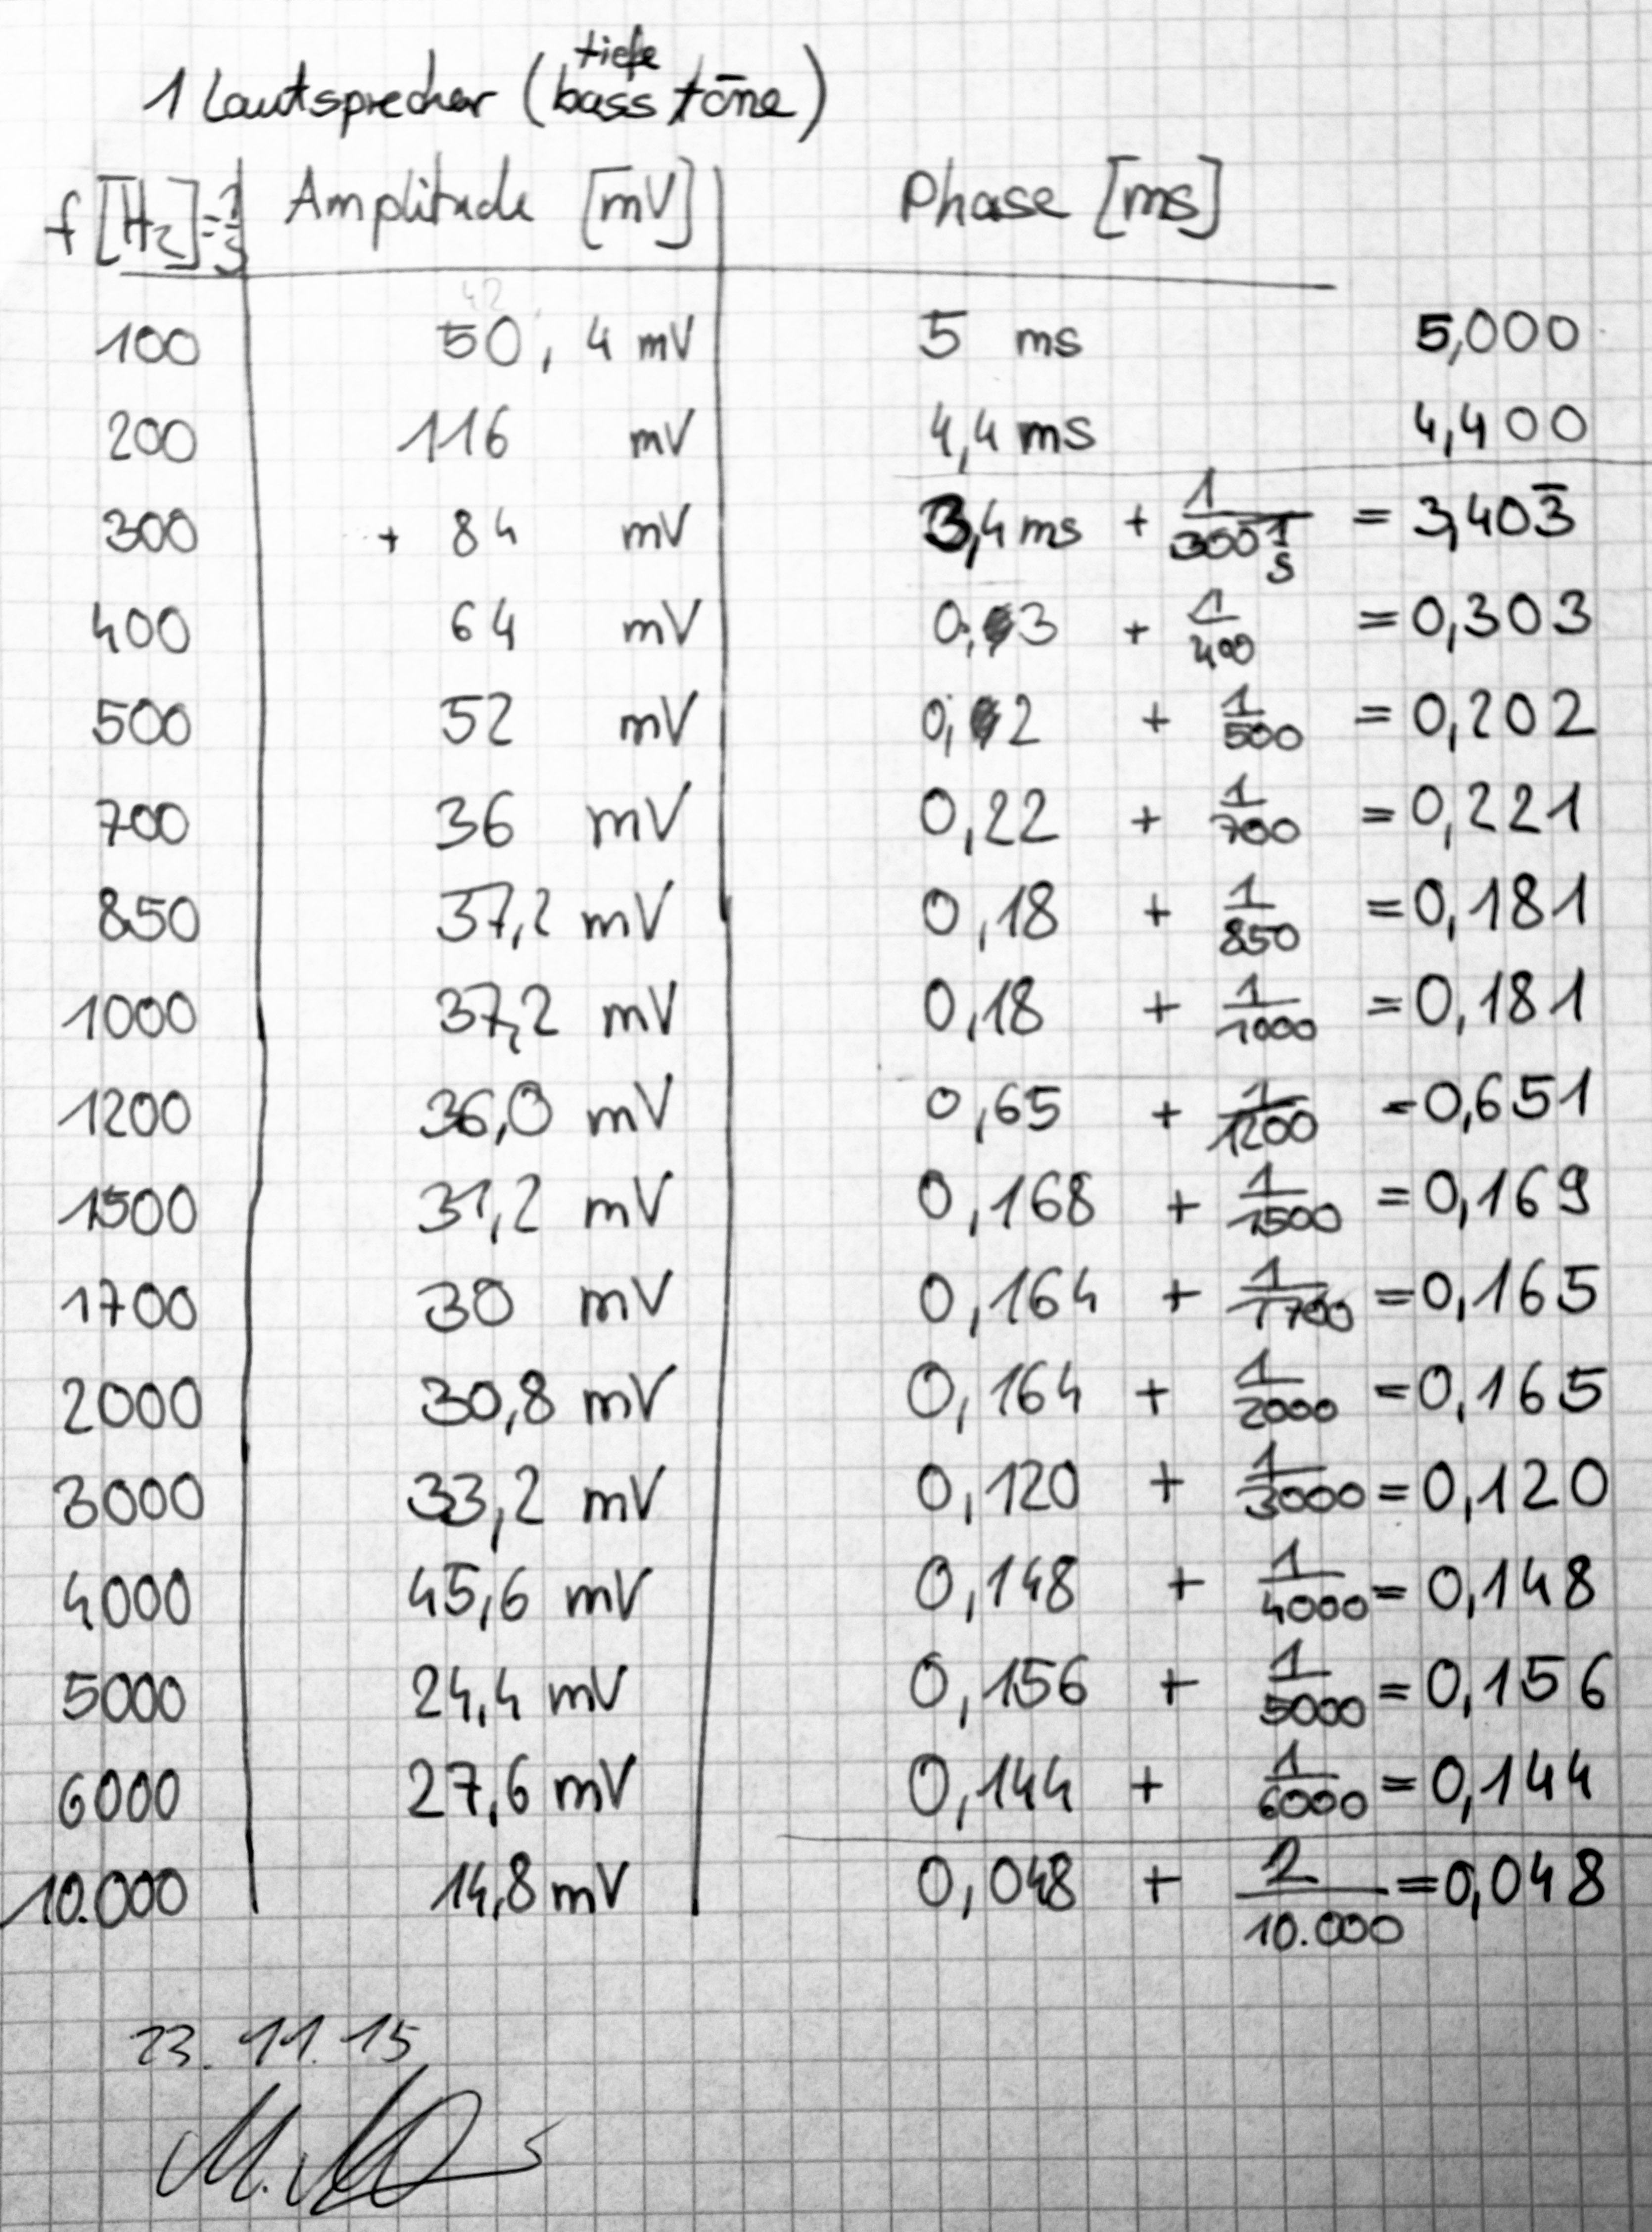
\includegraphics[scale=0.6]{src/1Lautsprecher_Messwerte.jpg}
\caption{Messwerte des großen Lautsprechers}
\label{fig:LAUT_TIEF}
\end{figure}

\begin{figure}
\centering\small
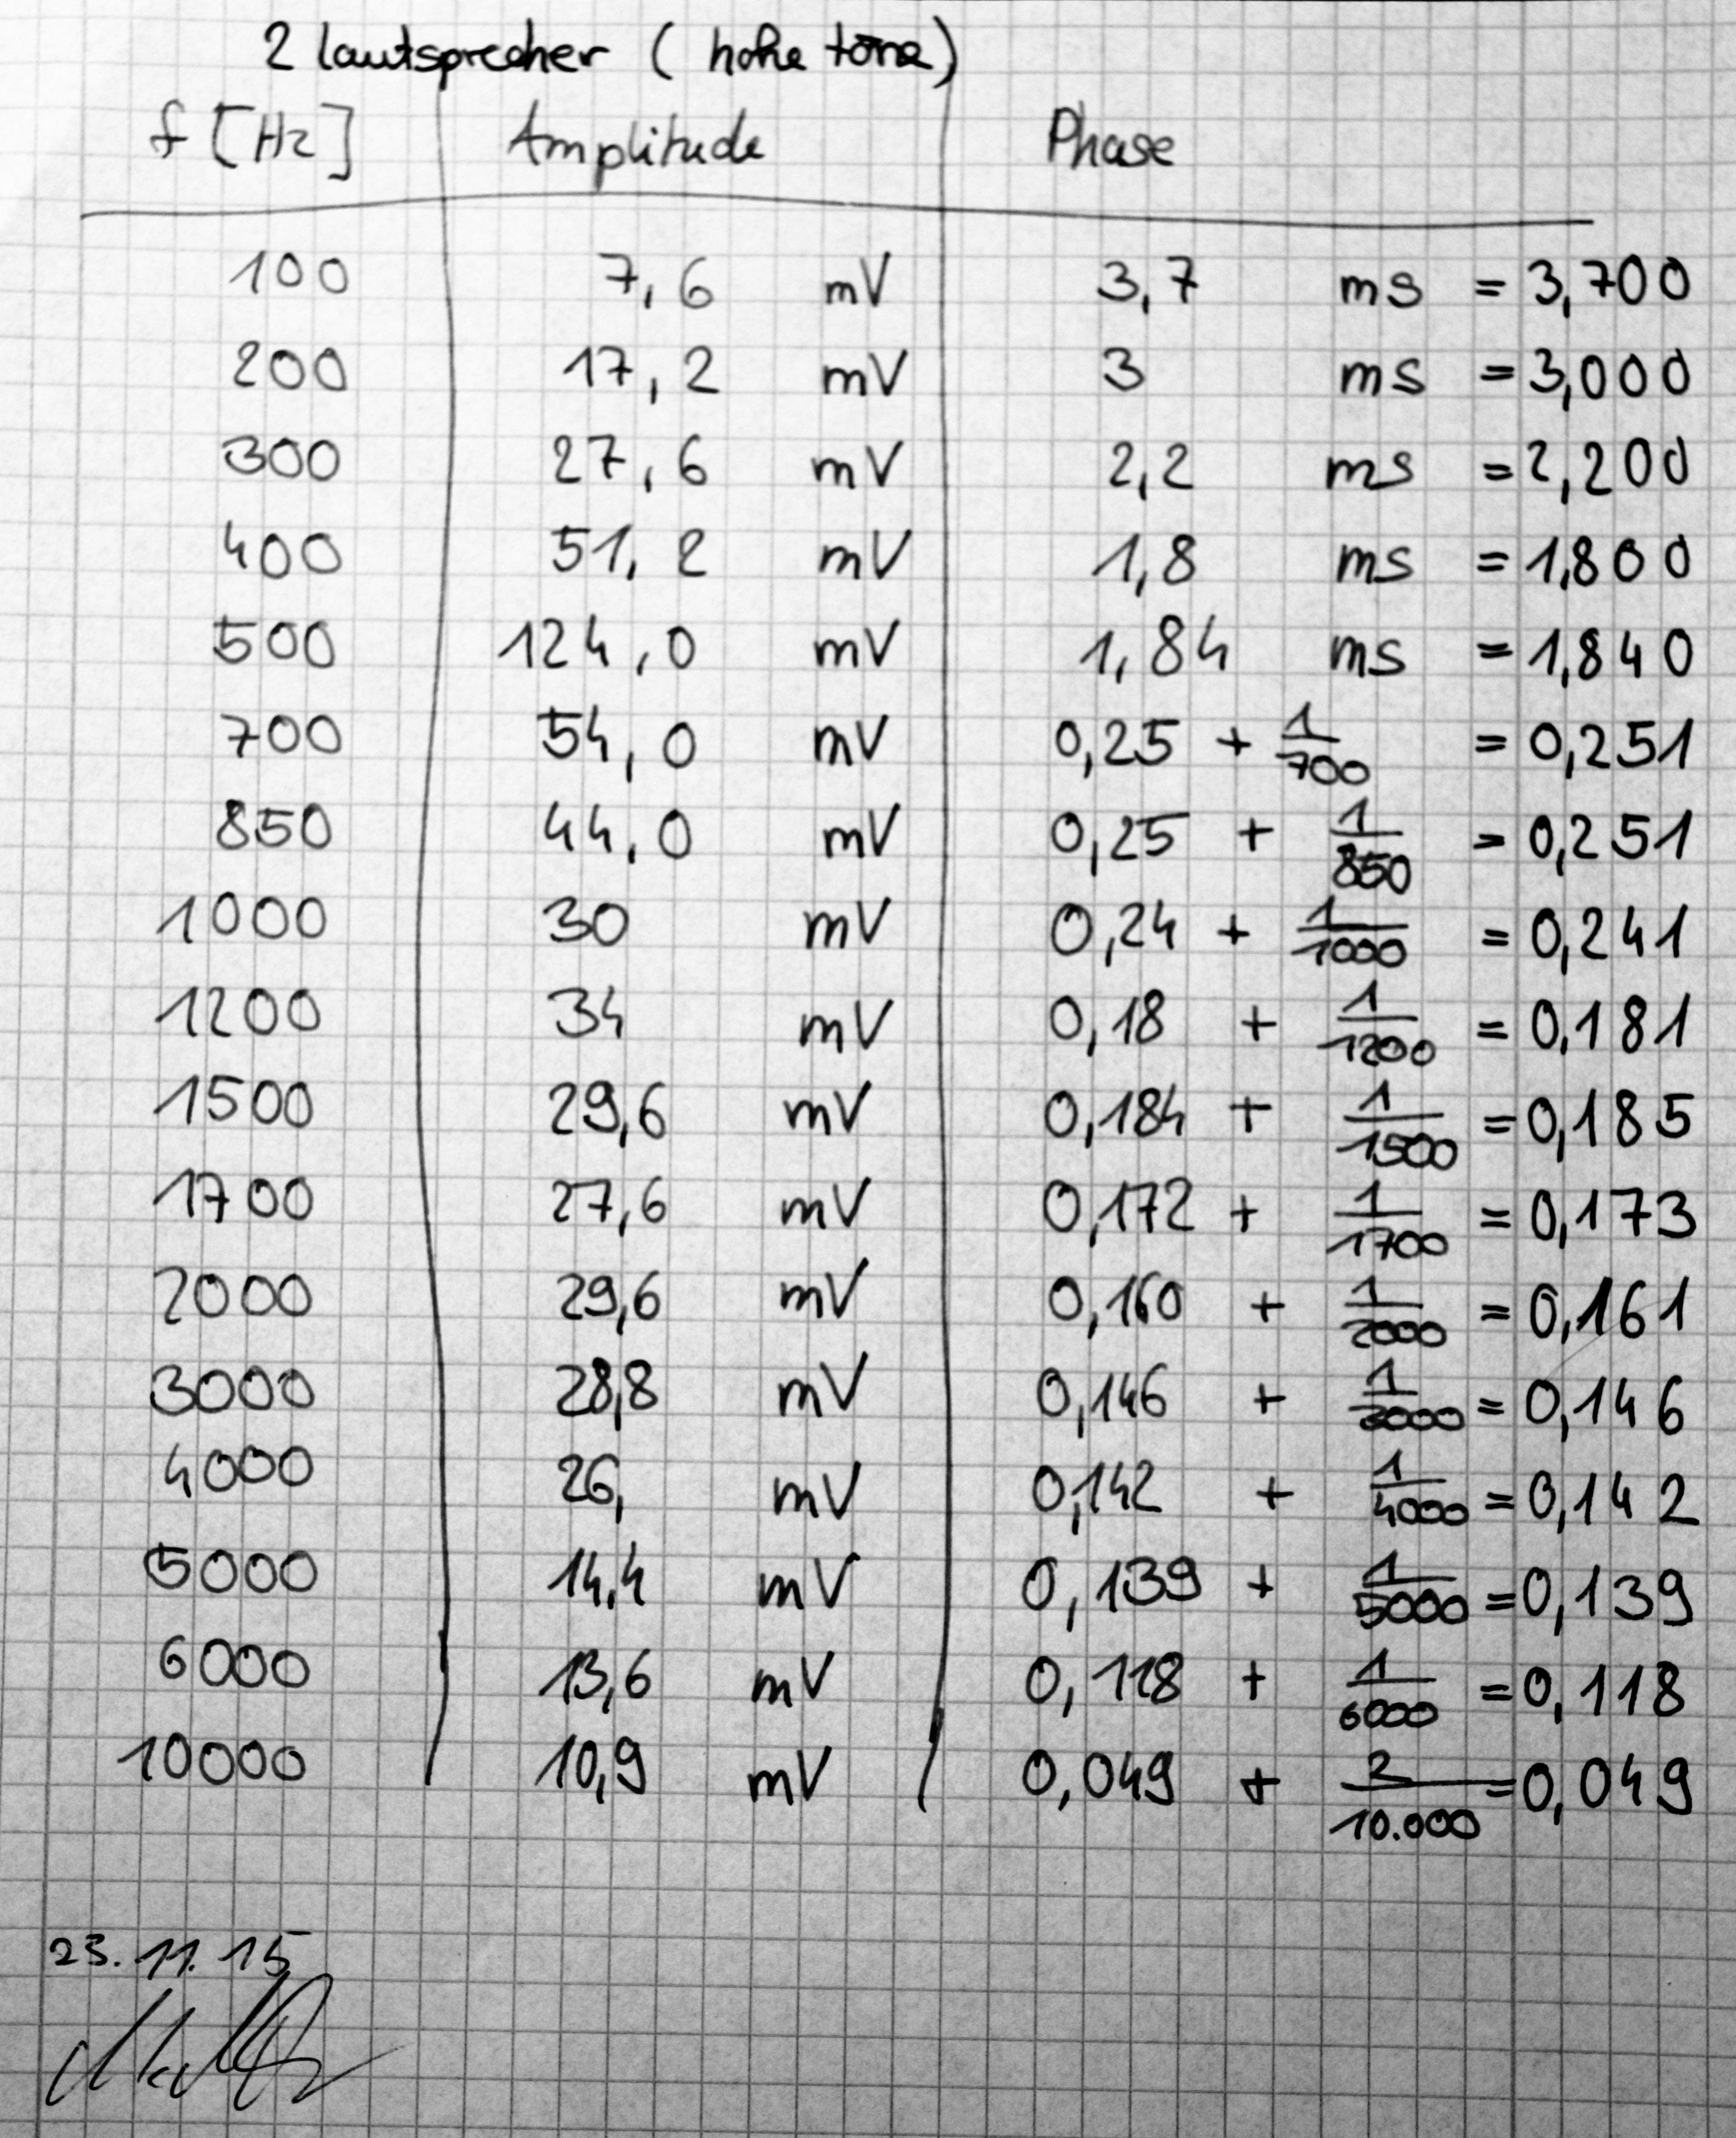
\includegraphics[scale=0.65]{src/2Lautsprecher_Messwerte.jpg}
\caption{Messwerte des kleinen Lautsprechers}
\label{fig:LAUT_HOCH}
\end{figure}

%
% Literaturverzeichnis
%
%
% Literaturverzeichnis
%
\phantomsection
\addcontentsline{toc}{chapter}{Literaturverzeichnis}
\bibliography{../references}
\newpage

\end{document}
%------------------------------------
% ╔═╗╔╗╔╔╦╗  ╔╦╗╔═╗╔═╗╦ ╦╔╦╗╔═╗╔╗╔╔╦╗
% ║╣ ║║║ ║║   ║║║ ║║  ║ ║║║║║╣ ║║║ ║ 
% ╚═╝╝╚╝═╩╝  ═╩╝╚═╝╚═╝╚═╝╩ ╩╚═╝╝╚╝ ╩ 
%------------------------------------